%=========================================================
% Capítulo 2 — Interpolação: o ponto de partida
%=========================================================
\chapter{Interpolação: o ponto de partida}
\label{ch:interpolacao}

\noindent\textbf{Resumo:}
Este capítulo introduz os fundamentos da interpolação como método de estimar valores em pontos desconhecidos a partir de dados observados. Apresenta exemplos de interpolação linear, polinomial e spline, discutindo seus limites e a motivação para evoluir em direção ao método dos mínimos quadrados. É aqui que nasce a noção de ``melhor estimativa'' em vez de ``ajuste exato''.

%---------------------------------------------------------
\section{Definição e motivação}
Interpolação é o processo de construir uma função contínua $f(x)$ que passa por um conjunto de pontos conhecidos $(x_i, y_i)$, $i = 1,2,\dots,n$.  
A forma mais simples é a \emph{interpolação linear}, que conecta os pontos por segmentos de reta:
\begin{equation}
f(x) = y_i + \frac{y_{i+1}-y_i}{x_{i+1}-x_i}\,(x-x_i), \quad x_i \le x \le x_{i+1}.
\label{eq:interp-linear}
\end{equation}
O resultado é uma aproximação por partes, contínua mas não suave nas junções.  
Quando se deseja uma função mais lisa, recorre-se à \emph{interpolação polinomial}.

%---------------------------------------------------------
\section{Interpolação polinomial}
Dado $n$ pontos, existe um polinômio de grau $n-1$ que os interpola exatamente:
\begin{equation}
P(x) = a_0 + a_1x + a_2x^2 + \dots + a_{n-1}x^{n-1}.
\label{eq:poly}
\end{equation}
Os coeficientes $a_k$ são determinados impondo $P(x_i)=y_i$.  
Por exemplo, para três pontos $(x_1,y_1)$, $(x_2,y_2)$ e $(x_3,y_3)$:
\begin{equation}
\begin{bmatrix}
1 & x_1 & x_1^2 \\
1 & x_2 & x_2^2 \\
1 & x_3 & x_3^2
\end{bmatrix}
\begin{bmatrix}
a_0 \\ a_1 \\ a_2
\end{bmatrix}
=
\begin{bmatrix}
y_1 \\ y_2 \\ y_3
\end{bmatrix}.
\label{eq:vandermonde}
\end{equation}
Essa é a \emph{matriz de Vandermonde}, cuja inversão dá a solução exata.  
Entretanto, quando o número de pontos aumenta, o polinômio tende a oscilar fortemente entre as amostras — o chamado \emph{efeito de Runge} — tornando-se inadequado para dados reais ruidosos.

%---------------------------------------------------------
\section{Interpolação por splines}
Para obter suavidade sem oscilações, utilizam-se \emph{splines}, especialmente o \emph{spline cúbico}, definido por polinômios de grau 3 em cada subintervalo $[x_i, x_{i+1}]$, com continuidade nas primeiras e segundas derivadas:
\[
S_i(x) = a_i + b_i(x-x_i) + c_i(x-x_i)^2 + d_i(x-x_i)^3.
\]
O spline cúbico oferece uma transição suave entre os pontos e é amplamente usado em aplicações meteorológicas, como interpolação de perfis verticais de temperatura e umidade.

%---------------------------------------------------------
\section{Limitações e surgimento do ajuste ótimo}
Na prática, medições contêm ruído e inconsistências. Se exigirmos que a função passe exatamente por todos os pontos, amplificamos os erros.  
O ideal é encontrar uma função que \emph{aproxime} os dados minimizando o erro global:
\begin{equation}
J(a_0,\dots,a_m) = \sum_{i=1}^{n} \big[y_i - f(x_i; a_0,\dots,a_m)\big]^2.
\label{eq:min-squares-cost}
\end{equation}
Essa função custo $J$ leva ao método dos \emph{mínimos quadrados}, que será formalmente desenvolvido no próximo capítulo. A interpolação, portanto, evolui naturalmente para o ajuste ótimo — uma transição conceitual essencial para a assimilação de dados, em que buscamos minimizar os erros entre o modelo e as observações.

%---------------------------------------------------------
\section{Figuras conceituais (pgfplots)}
As Figuras~\ref{fig:interp-linear} e \ref{fig:interp-poly} ilustram comparativamente a interpolação linear e polinomial entre cinco pontos.

\begin{figure}[h!]
\centering
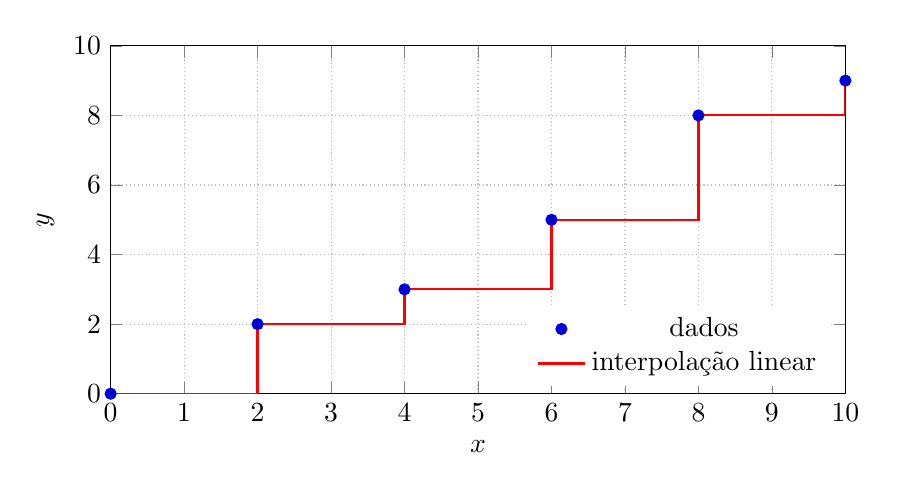
\begin{tikzpicture}
\begin{axis}[
  width=0.9\linewidth, height=6cm,
  xlabel={$x$}, ylabel={$y$},
  xmin=0, xmax=10, ymin=0, ymax=10,
  grid=both, grid style={densely dotted},
  legend style={at={(0.98,0.02)},anchor=south east,draw=none}
]
  % dados
  \addplot+[only marks,mark=*] coordinates {(0,0) (2,2) (4,3) (6,5) (8,8) (10,9)}; \addlegendentry{dados}
  % linear
  \addplot+[const plot, thick, mark=none] coordinates {(0,0) (2,2) (4,3) (6,5) (8,8) (10,9)};
  \addlegendentry{interpolação linear}
\end{axis}
\end{tikzpicture}
\caption{Interpolação linear por segmentos de reta: simples e contínua, mas não suave nas junções.}
\label{fig:interp-linear}
\end{figure}

\begin{figure}[h!]
\centering
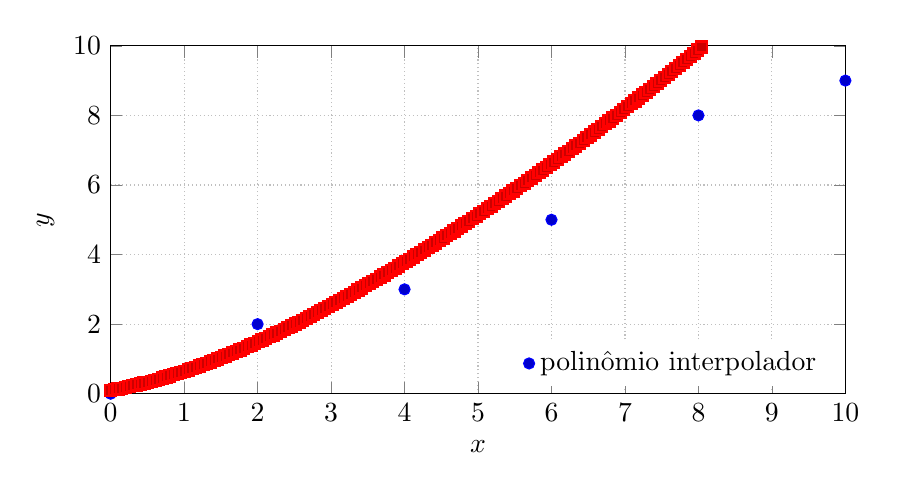
\begin{tikzpicture}
\begin{axis}[
  width=0.9\linewidth, height=6cm,
  xlabel={$x$}, ylabel={$y$},
  xmin=0, xmax=10, ymin=0, ymax=10,
  grid=both, grid style={densely dotted},
  legend style={at={(0.98,0.02)},anchor=south east,draw=none}
]
  \addplot+[only marks,mark=*] coordinates {(0,0) (2,2) (4,3) (6,5) (8,8) (10,9)};
  \addplot+[domain=0:10, samples=200, thick] {0.0007*x^4 - 0.016*x^3 + 0.19*x^2 + 0.37*x + 0.1};
  \addlegendentry{polinômio interpolador}
\end{axis}
\end{tikzpicture}
\caption{Interpolação polinomial de grau elevado: passa por todos os pontos, mas pode oscilar entre eles.}
\label{fig:interp-poly}
\end{figure}

%---------------------------------------------------------
\section{Síntese}
A interpolação é o ponto de partida natural da assimilação de dados: ambas buscam reconstruir um campo desconhecido a partir de informações discretas. Contudo, enquanto a interpolação tradicional busca o ajuste exato, a assimilação valoriza o equilíbrio entre coerência e confiança --- um ajuste \emph{ótimo} em vez de \emph{exato}. O passo seguinte é formalizar essa ideia através do método dos mínimos quadrados, que constitui o elo matemático entre interpolação e análise objetiva.

% Fim do Capítulo 2
